% Created 2021-05-30 Sun 21:06
% Intended LaTeX compiler: pdflatex
\documentclass[floatsintext,stu]{apa7}
\usepackage[utf8]{inputenc}
\usepackage[T1]{fontenc}
\usepackage{graphicx}
\usepackage{grffile}
\usepackage{longtable}
\usepackage{wrapfig}
\usepackage{rotating}
\usepackage[normalem]{ulem}
\usepackage{amsmath}
\usepackage{textcomp}
\usepackage{amssymb}
\usepackage{capt-of}
\usepackage{hyperref}
\shorttitle{PRODUCTION ANALYSIS}
\usepackage{hyperref}
\usepackage{fontawesome}
\usepackage{csquotes}
\usepackage{hhline}
\usepackage{colortbl}
\usepackage{arydshln}
\usepackage{caption}
\usepackage[utf8]{inputenc}
\usepackage[gen]{eurosym}
\usepackage[style=apa,sortcites=true,sorting=nyt,backend=biber]{biblatex}
\DeclareLanguageMapping{american}{american-apa}
\addbibresource{/home/david/Documents/School/References/bibliography.bib}
\affiliation{North Central University}
\course{TIM-8301: Principles of Cybersecurity}
\professor{Dr. Bill Souza}
\duedate{May 30, 2021}
\leftheader{Wagle}
\author{David A. Wagle}
\date{\today}
\title{Future of Supply Chain Security}
\hypersetup{
 pdfauthor={David A. Wagle},
 pdftitle={Future of Supply Chain Security},
 pdfkeywords={},
 pdfsubject={},
 pdfcreator={Emacs 27.2 (Org mode 9.5)}, 
 pdflang={English}}
\begin{document}

\maketitle


\section{Company and Blog Location}
\label{sec:org7ba9ef7}

\subsection{Company Name and URL}
\label{sec:orga69d0dc}

A.P. Moller - Maersk \url{https://maersk.com}

\subsection{Blog Post Location}
\label{sec:org785f5b5}

\url{https://dawworld.wordpress.com/2021/05/30/future-of-supply-chain-security/}

\newpage


\section{Introduction}
\label{sec:org8500567}

The supply chain is no longer simply about ordering supplies and maintaining inventories. Today, the supply chain represents the heart of a corporation's operational capability. A well-engineered supply chain is a significant, and often lasting, strategic advantage. Further, the supply chain is an extensive source of data, that can be leveraged using big-data analytics to support ever-more lean operations and economic efficiencies \cite{arunachalamUnderstandingBigData2018}.

The supply chain is also a major source of cybersecurity concerns. First, there is the very real issue that most supply chains contain some level of corruption which is ignored by the corporation \cite{webbTwoThirdsCorporationsIgnore2017}. Second, the simply reality is that the supply chain represents an enormous attack-surface for would-be attackers as the modern supply chain creates large deeply interconnected systems between multiple corporations \cite{govindanSupplyChainNetwork2017}.

Supply chain management (SCM) is focused on the integration of critical operational business processes to provide products, services, and information between companies connected in a supply chain relationship. In an end-to-end supply chain, there can be dozens of companies that are sharing data. The optimal supply chain, from an operational perspective, is highly flexible and dynamic. This flexibility, however, comes with a loss of control \cite{linawatiSupplyChainFlexibility2017}. Thus, the global supply chain becomes an ideal target for cyber-attackers wishing to create maximum havoc either for a particular company, industry, or nation.


\section{The Future of Risk Mitigation Might Be Now}
\label{sec:orgec4da04}

\subsection{Enter Blockchain}
\label{sec:orga9c77eb}

Consider a global shipping and logistics company: what are the cutting edge technologies currently being explored? The most famous new technology in such scenarios is blockchain  \cite{litkeBlockchainsSupplyChain2019}. Integration of blockchain into SCM systems for global logistics firms is already happening at a fairly rapid pace \cite{groenfeldtIBMMaerskApply2017}, although for smaller logistic and shipping firms, adoption can still be very low \cite{papathanasiouNonApplicationBlockchain2020}. One of the reasons for the low adoption rate is actually concerns about security. This is ironic, as blockchain technology offers an intriguing potential to increase both physical and cybersecurity in the shipping and logistics industry \cite{xuBindingPhysicalCyber2018}.

\subsection{What is Blockchain}
\label{sec:org987b9d5}

Simply put, blockchain is a technology for creating a shared database of transactions that can be trusted by all parties.

\begin{figure}[h]
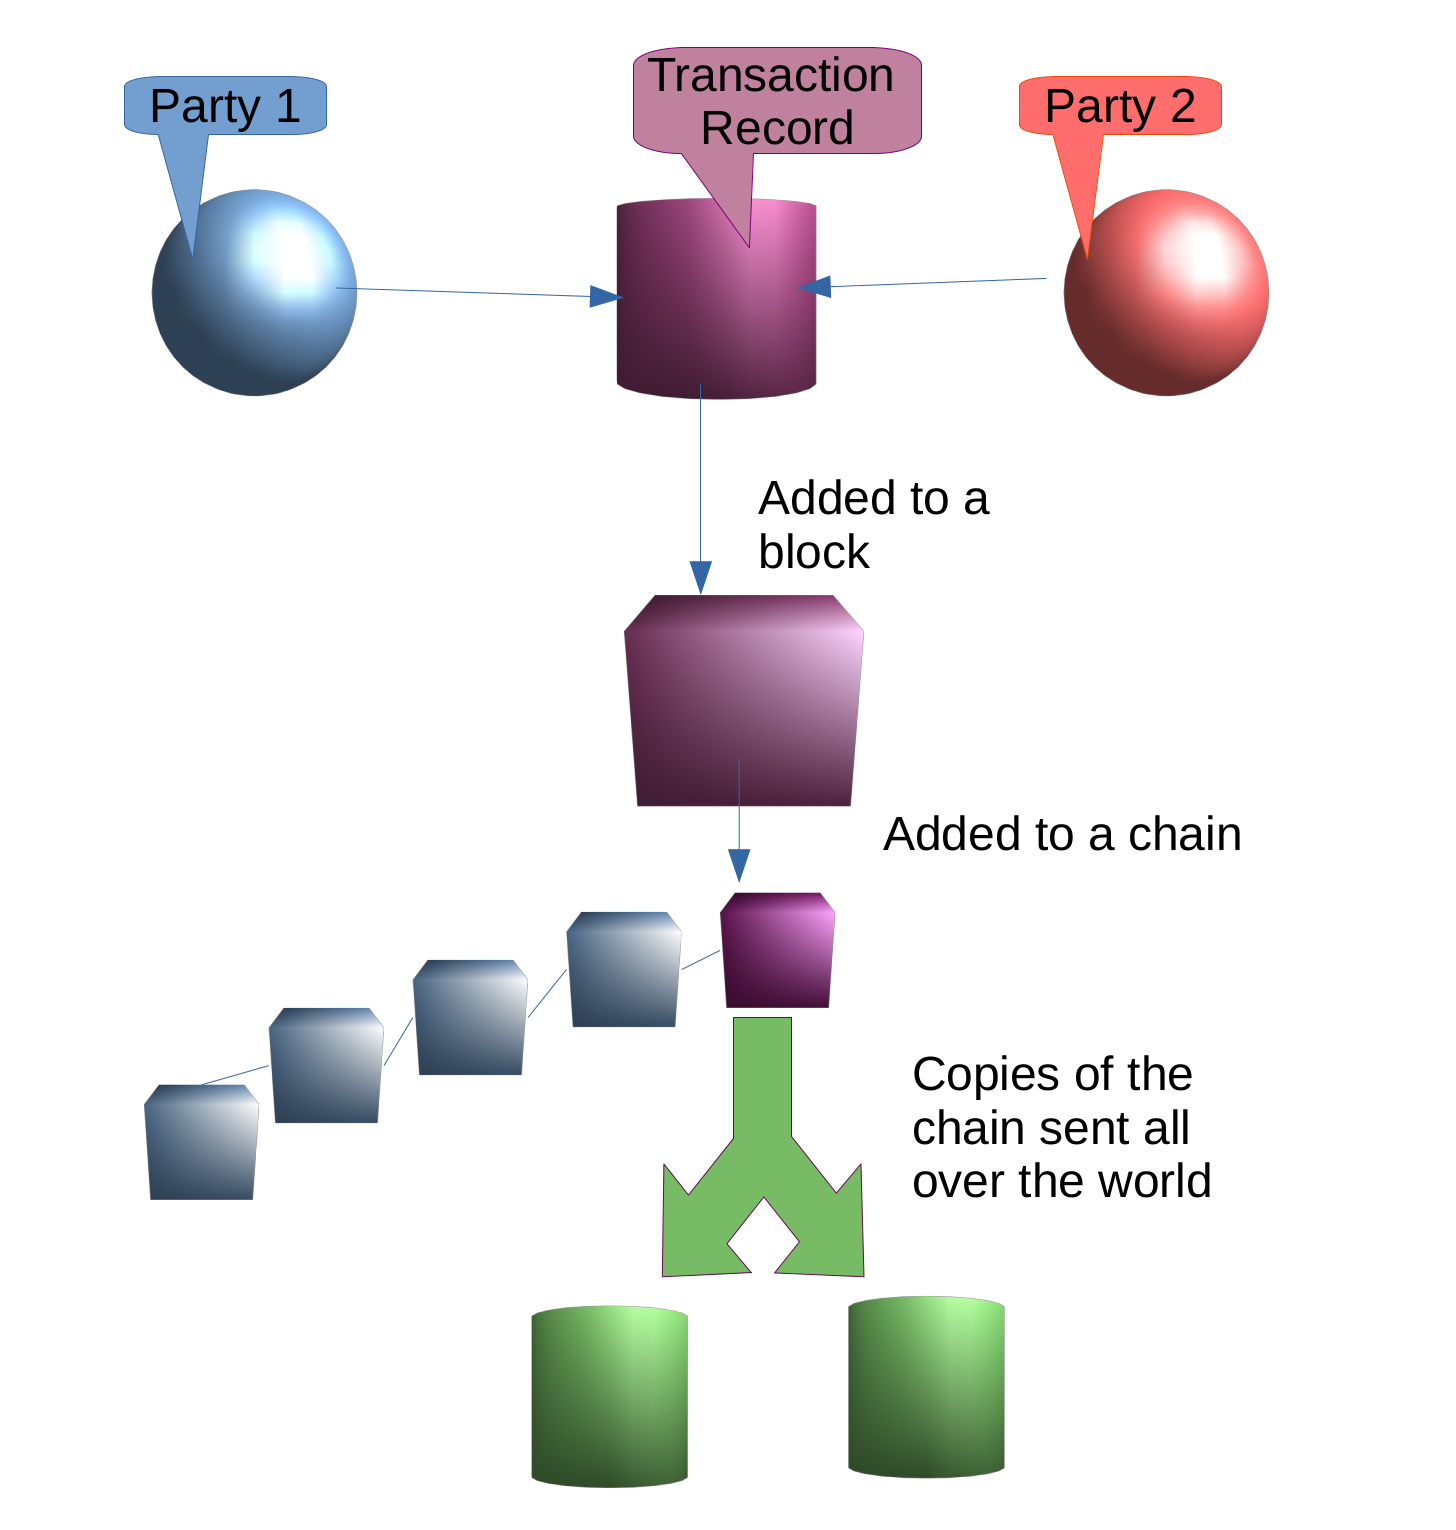
\includegraphics[width=.8\textwidth]{diagram}
\end{figure}


As the diagram suggests, a transaction is encoded into package called a block, that block is connected to other blocks on a chain, and the whole chain is then shared with many, many users around the world. The ``secret sauce'' that makes these transactions secure is two-fold. First, the transaction is encrypted using very strong encryption technologies that are virtually impossible to break. Second, and more important, the block is given a unique identifying number as it is added to the chain that is cryptographically guaranteed to be unalterable. Now, when the chain is shared to many users, the validity of the transaction and its place on the chain can be proven by having all holders of a copy of the chain ``vote'' to validate if a block belongs on the chain, and its place on the chain \cite{mearianWhatBlockchainComplete2019}.  

This public verification scheme makes a blockchain ledger virtually unalterable in practice. 

If the problem of adoption can be solved, and larger shipping and logistic companies are pushing that issue, supply chain security can be protected against malicious record alteration between suppliers, shippers, and end consumers. 

Without blockchain, the supply chain is open to record manipulation that allows cyber attackers to delete records, corrupt data, or even re-route shipments, allowing the cyber attackers to commit physical theft and fraud. With Blockchain, the security of the supply chain can be protected at scale across the globe. Proof of this concept has already been shown in a wide varity of industries from aggriculture to pharmaceuticals \cite{tseBlockchainApplicationFood2017}.

\printbibliography
\end{document}
